\documentclass[xcolor=dvipsnames]{beamer}

\usepackage[utf8]{inputenc}
\usepackage{multicol}
\usepackage{amssymb,amsmath,amsbsy,cmath} 
\usepackage{bm}    
\usepackage{graphicx,graphics,xcolor}
\usepackage{xcolor}
\usepackage{physics}
\usepackage{comment}
\usepackage{caption}
\usepackage[style=authortitle,backend=bibtex]{biblatex}
\addbibresource{References.bib}
\usepackage{yfonts}
\usepackage{pifont}


\newcommand\blfootnote[1]{%
  \begingroup
  \renewcommand\thefootnote{}\footcite{#1}%
  \addtocounter{footnote}{-1}%
  \endgroup
}


\usetheme{Madrid}
\useoutertheme{miniframes} % Alternatively: miniframes, infolines, split
\useinnertheme{circles}


\title[Schwartzschild geometry]{Schwartzschild Geometry: Static Black Holes}
\date{\today}
\author[Universidad del Valle]{Stiven Londoño}
\institute[]{Universidad del Valle \\ Departamento de física}

\begin{document}
	
	\begin{frame}
		\titlepage
	\end{frame}
	
	\begin{frame}{Table of contents}
    \tableofcontents
	\end{frame}
	
	
\section{Generalities}

\begin{frame}{Frame 1}

Para efectos de orden guardar imágenes como "4\_nombre.jpg/png/etc" en la carpeta "Images"

\begin{block}{Block 1}
\cite{hobson_efstathiou_lasenby_2006}    
\end{block}

\begin{figure}
    \centering
    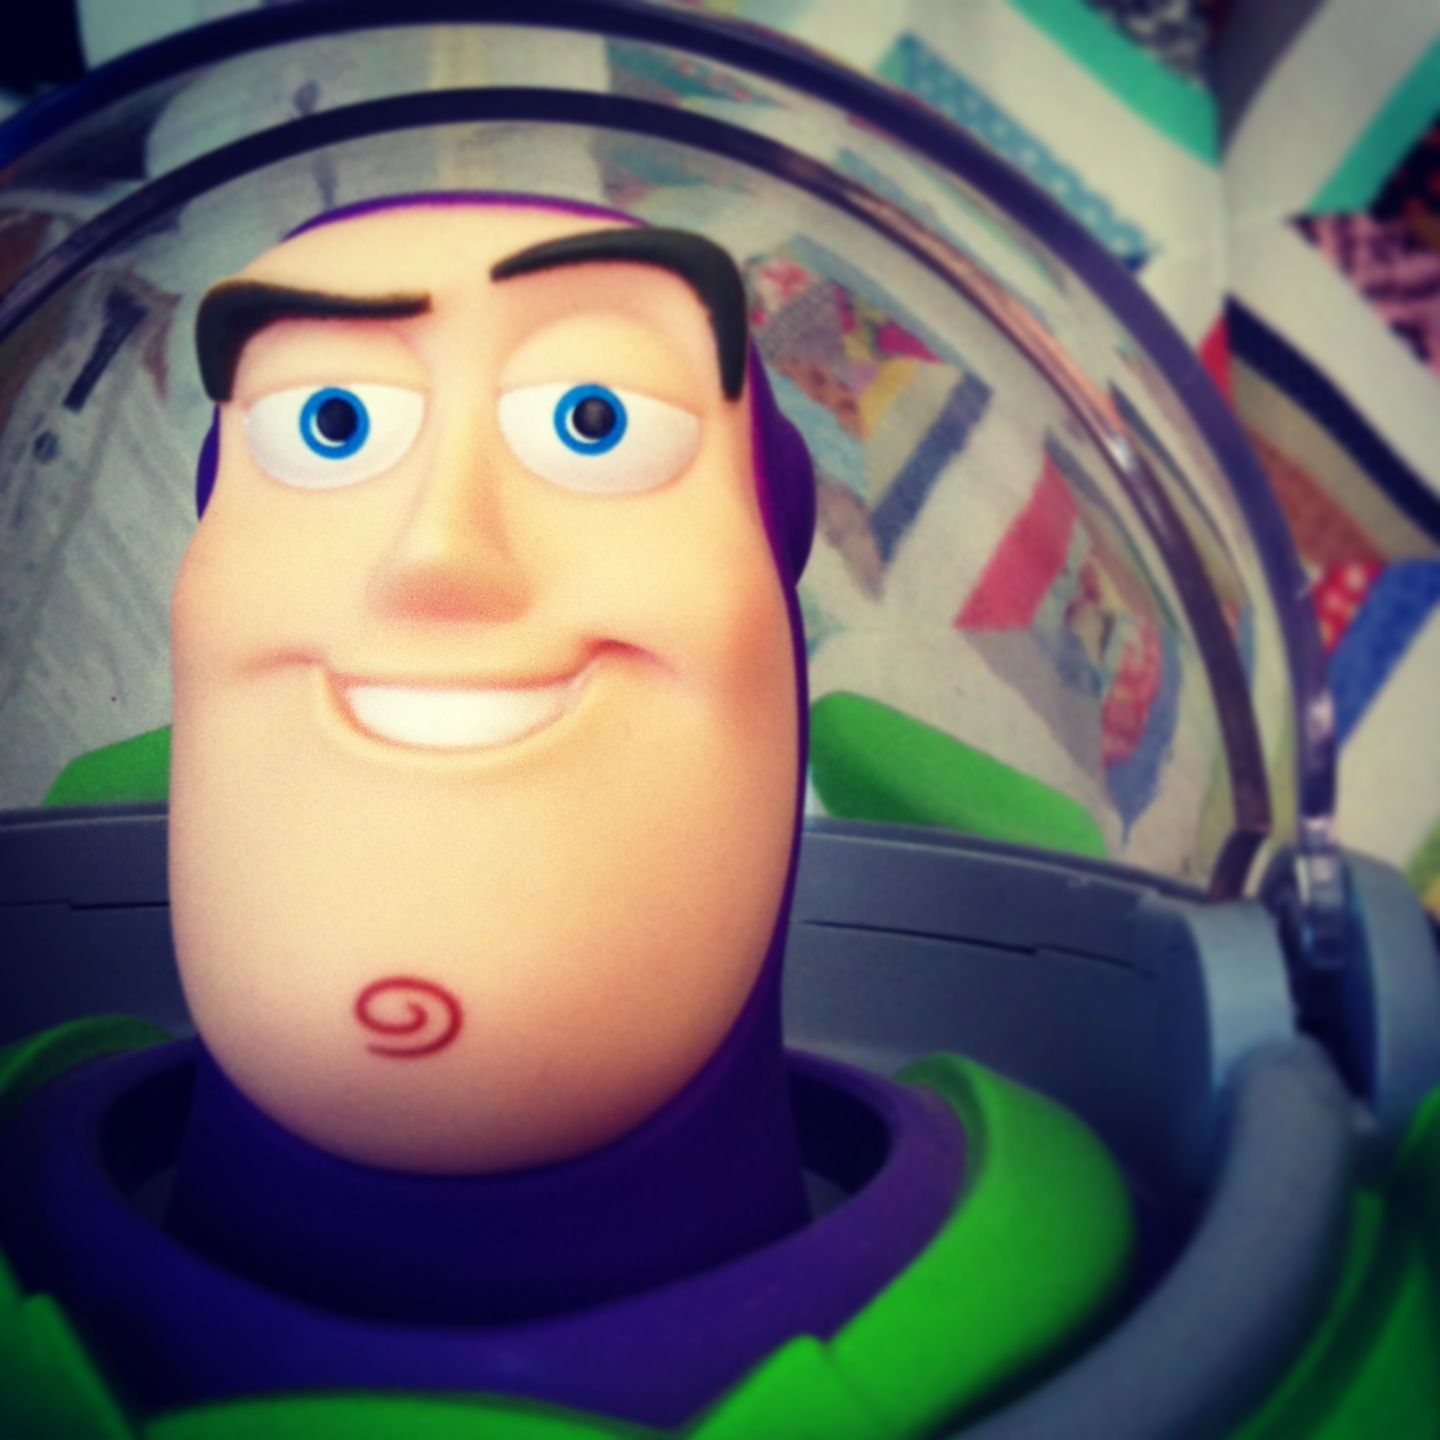
\includegraphics[width=0.25 \textwidth]{Presentations/Images/sample.jpg}
\end{figure}
    
\end{frame}

\section{Eddington-Finkelstein coordinates}
\begin{frame}{Frame 1}

\end{frame}

\begin{frame}{Frame 1}

\end{frame}




\begin{frame}{Frame 1}

\end{frame}
\section{Kruskal coordinates}


\begin{frame}{Frame 1}

\end{frame}



\begin{frame}{Frame 1}

\end{frame}
\end{document}